% Options for packages loaded elsewhere
\PassOptionsToPackage{unicode=true}{hyperref}
\PassOptionsToPackage{hyphens}{url}
%
\documentclass[
  ignorenonframetext,
]{beamer}
\usepackage{pgfpages}
\setbeamertemplate{caption}[numbered]
\setbeamertemplate{caption label separator}{: }
\setbeamercolor{caption name}{fg=normal text.fg}
\beamertemplatenavigationsymbolsempty
% Prevent slide breaks in the middle of a paragraph
\widowpenalties 1 10000
\raggedbottom
\setbeamertemplate{part page}{
  \centering
  \begin{beamercolorbox}[sep=16pt,center]{part title}
    \usebeamerfont{part title}\insertpart\par
  \end{beamercolorbox}
}
\setbeamertemplate{section page}{
  \centering
  \begin{beamercolorbox}[sep=12pt,center]{part title}
    \usebeamerfont{section title}\insertsection\par
  \end{beamercolorbox}
}
\setbeamertemplate{subsection page}{
  \centering
  \begin{beamercolorbox}[sep=8pt,center]{part title}
    \usebeamerfont{subsection title}\insertsubsection\par
  \end{beamercolorbox}
}
\AtBeginPart{
  \frame{\partpage}
}
\AtBeginSection{
  \ifbibliography
  \else
    \frame{\sectionpage}
  \fi
}
\AtBeginSubsection{
  \frame{\subsectionpage}
}
\usepackage{lmodern}
\usepackage{amssymb,amsmath}
\usepackage{ifxetex,ifluatex}
\ifnum 0\ifxetex 1\fi\ifluatex 1\fi=0 % if pdftex
  \usepackage[T1]{fontenc}
  \usepackage[utf8]{inputenc}
  \usepackage{textcomp} % provides euro and other symbols
\else % if luatex or xelatex
  \usepackage{unicode-math}
  \defaultfontfeatures{Scale=MatchLowercase}
  \defaultfontfeatures[\rmfamily]{Ligatures=TeX,Scale=1}
\fi
% Use upquote if available, for straight quotes in verbatim environments
\IfFileExists{upquote.sty}{\usepackage{upquote}}{}
\IfFileExists{microtype.sty}{% use microtype if available
  \usepackage[]{microtype}
  \UseMicrotypeSet[protrusion]{basicmath} % disable protrusion for tt fonts
}{}
\makeatletter
\@ifundefined{KOMAClassName}{% if non-KOMA class
  \IfFileExists{parskip.sty}{%
    \usepackage{parskip}
  }{% else
    \setlength{\parindent}{0pt}
    \setlength{\parskip}{6pt plus 2pt minus 1pt}}
}{% if KOMA class
  \KOMAoptions{parskip=half}}
\makeatother
\usepackage{xcolor}
\IfFileExists{xurl.sty}{\usepackage{xurl}}{} % add URL line breaks if available
\IfFileExists{bookmark.sty}{\usepackage{bookmark}}{\usepackage{hyperref}}
\hypersetup{
  pdftitle={RMarkdown and Bookdown for Academic Writing in R},
  pdfauthor={Thea Knowles, R-Ladies \#LdnOnt},
  hidelinks,
}
\urlstyle{same} % disable monospaced font for URLs
\newif\ifbibliography
\usepackage{longtable,booktabs}
\usepackage{caption}
% Make caption package work with longtable
\makeatletter
\def\fnum@table{\tablename~\thetable}
\makeatother
\usepackage{graphicx,grffile}
\makeatletter
\def\maxwidth{\ifdim\Gin@nat@width>\linewidth\linewidth\else\Gin@nat@width\fi}
\def\maxheight{\ifdim\Gin@nat@height>\textheight\textheight\else\Gin@nat@height\fi}
\makeatother
% Scale images if necessary, so that they will not overflow the page
% margins by default, and it is still possible to overwrite the defaults
% using explicit options in \includegraphics[width, height, ...]{}
\setkeys{Gin}{width=\maxwidth,height=\maxheight,keepaspectratio}
\setlength{\emergencystretch}{3em} % prevent overfull lines
\providecommand{\tightlist}{%
  \setlength{\itemsep}{0pt}\setlength{\parskip}{0pt}}
\setcounter{secnumdepth}{-\maxdimen} % remove section numbering

% Set default figure placement to htbp
\makeatletter
\def\fps@figure{htbp}
\makeatother


\title{RMarkdown and Bookdown for Academic Writing in R}
\author{Thea Knowles, R-Ladies \#LdnOnt}
\date{January 14, 2020}

\begin{document}
\frame{\titlepage}

\begin{frame}{Writing reports and manuscripts in R Markdown}
\protect\hypertarget{writing-reports-and-manuscripts-in-r-markdown}{}

\begin{block}{Agenda}

We will create the following files: - Helper R script (helper.R) -
Summary report (starwars\_summary.Rmd) - Manuscript 1
(starwars\_manuscript1.Rmd) - Manuscript 2 (starwars\_manuscript2.Rmd) -
Thesis (starwars\_thesis.Rmd)

\end{block}

\begin{block}{Why R Markdown?}

\begin{itemize}
\tightlist
\item
  Integrate data, code directly into writing
\item
  Reference management integration
\item
  Reproducibility
\item
  Accessible learning curve
\end{itemize}

\url{https://rmarkdown.rstudio.com/}

\end{block}

\begin{block}{Why bookdown?}

\begin{itemize}
\tightlist
\item
  Integrate multiple R Markdown documents into a larger project
\item
  Keep chapters separate
\end{itemize}

\url{https://bookdown.org/yihui/bookdown/}

\end{block}

\begin{block}{Knitting}

When you run R Markdown, you are \textbf{knitting} together plain
Markdown text and R code.

\end{block}

\end{frame}

\begin{frame}{Getting set up}
\protect\hypertarget{getting-set-up}{}

\begin{block}{Installation}

\begin{block}{Have installed the following software}

Required:

\begin{itemize}
\tightlist
\item
  \href{https://cran.r-project.org/}{R}
\item
  \href{rstudio.com}{RStudio}
\end{itemize}

\end{block}

\end{block}

\begin{block}{Installation}

Other software to be aware of:

\begin{itemize}
\tightlist
\item
  \href{https://pandoc.org/installing.html}{Pandoc}

  \begin{itemize}
  \tightlist
  \item
    If you have RStudio installed, Pandoc is automatically installed too
  \item
    Pandoc does the converting from .Rmd to .md, .docx, .pdf, .html,
    etc.
  \item
    It's working hard behind the scenes, but we don't interact with it
    too much
  \end{itemize}
\item
  \href{https://www.latex-project.org/get/}{Latex}

  \begin{itemize}
  \tightlist
  \item
    Necessary to install if you want to output PDFs
  \item
    We won't do this today
  \end{itemize}
\end{itemize}

\end{block}

\end{frame}

\begin{frame}[fragile]{RProjects}
\protect\hypertarget{rprojects}{}

\begin{block}{EXERCISE 1 \textbar{} Make a new R Project for this
workshop}

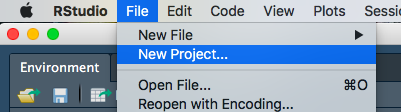
\includegraphics{images/new_project.png}

\begin{itemize}
\tightlist
\item
  Make a new directory for this workshop
\item
  Put the workshop contents in the same directory
\end{itemize}

\end{block}

\begin{block}{Install the following packages}

Copy and paste this code into your R console and run it

\begin{itemize}
\tightlist
\item
  \texttt{install.packages(c("rmarkdown","knitr","bookdown"))}
\item
  You can also do this manually in the Packages pane
\end{itemize}

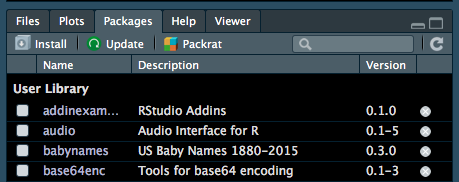
\includegraphics{images/packages_pane.png}

\end{block}

\begin{block}{Create a new R Markdown file}

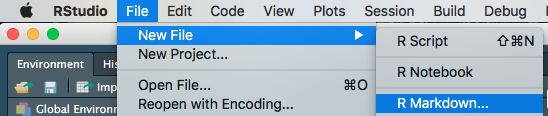
\includegraphics{images/new_rmarkdown1.png}

\end{block}

\begin{block}{EXCERCISE 1 \textbar{} Recap}

\begin{enumerate}
\tightlist
\item
  Make new R Project
\item
  \texttt{install.packages(c("rmarkdown","knitr","bookdown"))}
\item
  Creat new R Markdown document
\end{enumerate}

\end{block}

\begin{block}{Essential parts of any R Markdown document}

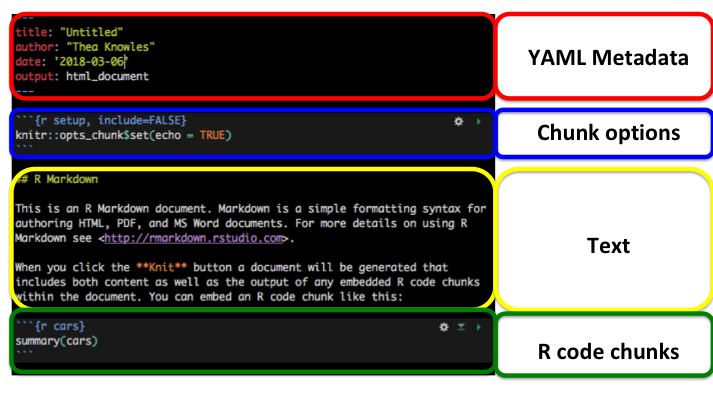
\includegraphics{images/rmarkdown_parts.png}

\end{block}

\begin{block}{YAML}

\href{https://en.wikipedia.org/wiki/YAML}{YAML} (rhymes with camel): The
header that tells R Markdown how to generate your document. Indentation
and spacing are very important.

\begin{itemize}
\tightlist
\item
  Permits the following to happen when you knit:

  \begin{itemize}
  \tightlist
  \item
    .Rmd -\textgreater{} knitr -\textgreater{} .md -\textgreater{}
    Pandoc -\textgreater{} output
  \item
    Output can be .docx, .html, .pdf, and many others
  \end{itemize}
\item
  YAML: ``YAML Ain't Markup Language''
\end{itemize}

\textbf{Basic: }

\begin{verbatim}
title: "Untitled"
author: "Thea Knowles"
date: '2018-02-18'
output: word_document
\end{verbatim}

\end{block}

\begin{block}{YAML}

\textbf{Gettin' fancy}

\begin{verbatim}
title: "A very important title"
subtitle: "A less important subtitle"
author:
     name: Thea Knowles
     affiliation: Western University
     name: Scott Adams
     affiliation: Western University
     affiliation: University Hospital
date: "11 January, 2020"
\end{verbatim}

\end{block}

\begin{block}{YAML}

\textbf{Even fancier:}

\begin{itemize}
\tightlist
\item
  output extensions
\item
  template
\item
  bibliography file
\item
  csl (references style guide)
\item
  css (supreme customization!)
\end{itemize}

\textbf{Different options for:}

\begin{itemize}
\tightlist
\item
  \href{https://rmarkdown.rstudio.com/html_document_format.html}{HTML
  output}
\item
  \href{https://rmarkdown.rstudio.com/word_document_format.html}{Word
  output}
\item
  \href{https://rmarkdown.rstudio.com/pdf_document_format.html}{PDF
  output}
\end{itemize}

\end{block}

\begin{block}{Essential parts of any R Markdown document}

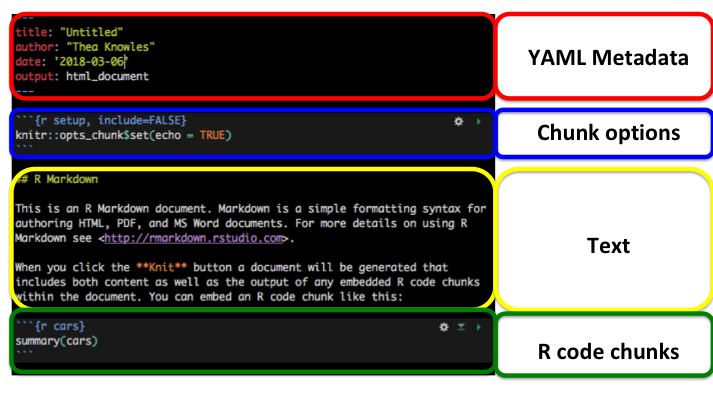
\includegraphics{images/rmarkdown_parts.png}

\end{block}

\begin{block}{Set chunk options}

\begin{itemize}
\tightlist
\item
  \href{http://yihui.name/knitr/options/}{\emph{Chunks}} are sections
  that will include R code. By setting defaults at the beginning of your
  document, you can specify what you want most of your chunks to do.
\item
  In each chunk, you can specify options in the form \texttt{tag=value}
  in the chunk header.

  \begin{itemize}
  \tightlist
  \item
    For example, in the following, the tag \texttt{include} is set to
    \texttt{FALSE}, indicating that we don't want the contents of this
    chunk included in the output
  \end{itemize}
\end{itemize}

This is the default chunk options set when you create a new .RMD (R
Markdown) file.

\begin{verbatim}
```{r setup, include=FALSE}
knitr::opts_chunk$set(echo = TRUE)
```
\end{verbatim}

\end{block}

\begin{block}{Set chunk options}

\begin{verbatim}
```{r setup, include=FALSE}
knitr::opts_chunk$set(echo = TRUE)
```
\end{verbatim}

This chunk provides the following information for ``knitting'' the
document:

\begin{itemize}
\tightlist
\item
  \texttt{setup}: the name of the chunk You shouldn't have two chunks
  with the same name, unless they are unnamed (in which case they just
  get numbered automatically during the knit process)
\item
  \texttt{include\ =\ false}: the chunk will not be included in the
  output after knitting.
\item
  \texttt{knitr::opts\_chunk\$set(echo\ =\ TRUE)}: the default behavior
  for chunks is to ``echo;'' you will see the actual code printed in the
  final output. You can set this to false if you don't want the actual
  code included by default.
\end{itemize}

\end{block}

\begin{block}{Set chunk options}

\begin{itemize}
\tightlist
\item
  You don't have to change this unless you want to
\item
  You can assign different values on a chunk-by-chunk basis
\item
  More on this in a minute!
\end{itemize}

\end{block}

\begin{block}{Essential parts of any R Markdown document}

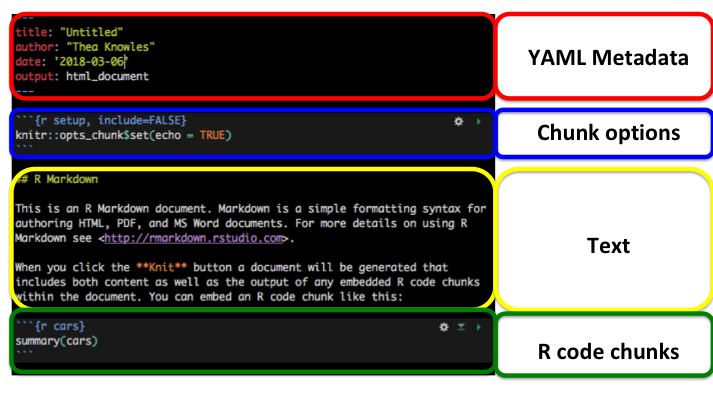
\includegraphics{images/rmarkdown_parts.png}

\end{block}

\begin{block}{Text in R Markdown \textbar{} The briefest intro to
Markdown syntax}

\begin{itemize}
\tightlist
\item
  \href{https://www.rstudio.com/wp-content/uploads/2016/03/rmarkdown-cheatsheet-2.0.pdf}{R
  Markdown Cheat Sheet}
\item
  \href{https://www.rstudio.com/wp-content/uploads/2016/03/rmarkdown-cheatsheet-2.0.pdf}{R
  Markdown Reference Guide}
\end{itemize}

\end{block}

\begin{block}{Essential parts of any R Markdown document}

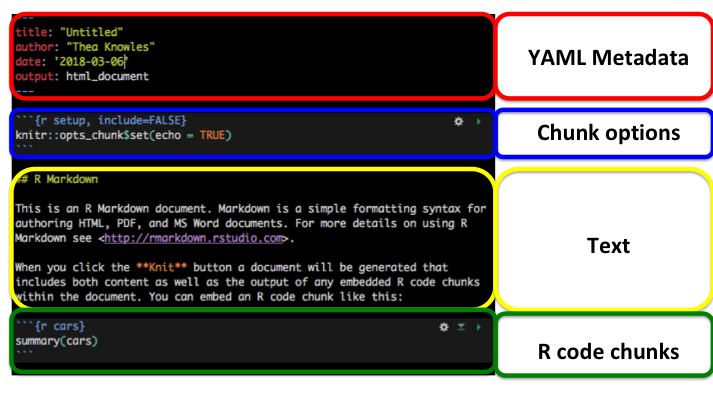
\includegraphics{images/rmarkdown_parts.png}

\end{block}

\begin{block}{R code chunks}

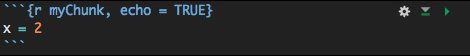
\includegraphics{images/mychunk.png}

\begin{itemize}
\tightlist
\item
  Insert chunks: cmd + k or click
  \texttt{Code\ \textgreater{}\textgreater{}\ Insert\ chunk}
\item
  name your chunk (\texttt{myChunk})
\item
  specify options (\texttt{echo=TRUE})
\end{itemize}

Some other options

\begin{itemize}
\tightlist
\item
  \texttt{echo\ =\ FALSE}: don't show the code itself in the final
  document
\item
  \texttt{include\ =\ FALSE}: don't include this code or its output in
  the final document
\item
  \texttt{eval\ =\ FALSE}: don't actually run this code at all
\item
  \href{https://yihui.name/knitr/options/}{And more\ldots{}}
\end{itemize}

\end{block}

\end{frame}

\begin{frame}[fragile]{Before we begin}
\protect\hypertarget{before-we-begin}{}

\begin{block}{Recipe for R Markdown summary document \textbar{} My
suggestion}

\begin{longtable}[]{@{}cc@{}}
\toprule
Ingredient & In this example\tabularnewline
\midrule
\endhead
data & starbucks\_drinkMenu\_expanded.csv\tabularnewline
helper script & helper.R\tabularnewline
R Markdown summary document &
preliminary\_results\_summary.Rmd\tabularnewline
\bottomrule
\end{longtable}

\end{block}

\begin{block}{1. Data}

\texttt{starbucks\_drinkMenu\_expanded.csv}

\begin{itemize}
\tightlist
\item
  We will use the same data Pierina used in her October Intro to R
  workshop (from kaggle.com)

  \begin{itemize}
  \tightlist
  \item
    Redundancy = good!
  \item
    Thea = lazy
  \end{itemize}
\item
  \href{https://www.meetup.com/rladies-ldnont/messages/boards/thread/51164998}{Check
  out Pierina's materials for a refresher}
\end{itemize}

\end{block}

\begin{block}{2. Helper script}

\texttt{helper.R}

\begin{itemize}
\tightlist
\item
  Use a helper .R script to do your data cleaning and basic analyses
\item
  Straight up R code. No markdown.
\item
  You can pull this .R document into future .RMD documents using
  \texttt{source()}
\item
  The benefit of using a helper script is that you can keep your
  analyses consistant. Whether you're writing an informal summary report
  to share with your supervisor or a full manuscript, you don't have to
  copy and paste the analyses each time you do something new.
\end{itemize}

\end{block}

\begin{block}{3. R Markdown document}

\begin{itemize}
\tightlist
\item
  \texttt{preliminary\_results\_summary.Rmd}
\end{itemize}

\begin{block}{R Markdown documents\ldots{}}

\begin{itemize}
\tightlist
\item
  End in extension \texttt{.Rmd}
\item
  Incorporate both R code (in chunks) and plain text (in Markdown)
\item
  Require YAML at the beginning
\end{itemize}

\end{block}

\end{block}

\end{frame}

\begin{frame}{Let's get started!}
\protect\hypertarget{lets-get-started}{}

\end{frame}

\begin{frame}{1. Make a new R Project for this workshop \textbar{}
DONE!}
\protect\hypertarget{make-a-new-r-project-for-this-workshop-done}{}

\end{frame}

\begin{frame}[fragile]{2. Write helper .R script}
\protect\hypertarget{write-helper-.r-script}{}

\begin{block}{2. Write helper .R script}

\begin{block}{Create a helper script as you would a regular R script}

\begin{itemize}
\tightlist
\item
  Open your new RProj file, which will start a new RStudio Session
\item
  Create and save a new R script entitled (for example) helper.R
\item
  Include the code you'd use to load in your data, tidy it up, analyze
  it, and visualize it

  \begin{itemize}
  \tightlist
  \item
    You can edit more of this code when you're writing your reports, too
  \end{itemize}
\end{itemize}

\textbf{For now:} Just open helper.R - Let's review it briefly 📚

\end{block}

\end{block}

\begin{block}{EXERCISE 2 \textbar{} Run helper.R}

\begin{itemize}
\tightlist
\item
  Open helper.R
\item
  Select all text and type \texttt{command\ +\ R} OR click Run (top
  right of script pane)
\item
  You can also run each line one at a time by clicking
  \texttt{command\ +\ R}
\end{itemize}

\emph{Got an error?}

\begin{itemize}
\tightlist
\item
  You may need to install packages first (see the comments in helper.R)
\end{itemize}

\end{block}

\begin{block}{Need a refresher on other skills in R? \textbar{} Check
out our past R-Ladies' presentations!}

\begin{itemize}
\tightlist
\item
  Need a refresher on\ldots{}

  \begin{itemize}
  \tightlist
  \item
    Scripting? Check out
    \href{https://www.meetup.com/rladies-ldnont/messages/boards/thread/51239206}{Rachael's
    materials!}
  \item
    Loading in your data? Check out
    \href{https://www.meetup.com/rladies-ldnont/messages/boards/thread/51164998}{Pierina's
    intros}
  \item
    Data visualization? See\ldots{}

    \begin{itemize}
    \tightlist
    \item
      \href{https://www.meetup.com/rladies-ldnont/messages/boards/thread/50724440}{Sinthiya's
      data visualization materials}
    \item
      \href{https://www.meetup.com/rladies-ldnont/messages/boards/thread/50864967}{Olivia's
      materials on 2d and 3d graphics}
    \end{itemize}
  \item
    Analyses? See\ldots{}

    \begin{itemize}
    \tightlist
    \item
      \href{https://www.meetup.com/rladies-ldnont/messages/boards/thread/50910795}{Monica's
      data manip \& multivariate analyses}
    \item
      \href{https://drive.google.com/drive/folders/0BznwYF956_rDRUtoS3N4dldySmc?usp=sharing}{Daryn's
      SPSS to R stats code}
    \item
      \href{https://www.meetup.com/rladies-ldnont/messages/boards/thread/51292341}{Jaky's
      regression materials}
    \end{itemize}
  \end{itemize}
\end{itemize}

\end{block}

\end{frame}

\begin{frame}[fragile]{3. Writing a summary report}
\protect\hypertarget{writing-a-summary-report}{}

\begin{block}{Got my data in! 💃}

\end{block}

\begin{block}{Gotta tell all my friends! 🎉}

\emph{i.e., gotta report it to my supervisor}

\end{block}

\begin{block}{3. Writing a summary report}

\begin{block}{\textbf{From scratch: }}

Make a new R Markdown document and store it in the same directory as
your helper.R script

\end{block}

\begin{block}{\textbf{For now:}}

Just open \texttt{preliminary\_results\_summary.Rmd}

\begin{itemize}
\tightlist
\item
  Let's review it briefly 📚
\end{itemize}

\end{block}

\end{block}

\begin{block}{3. Writing a summary report}

\begin{block}{Notice our YAML and chunk options!}

\begin{itemize}
\tightlist
\item
  These are the defaults that are included when you generate a new .Rmd
  file (I haven't changed them)
\item
  We'll leave the defaults in the YAML and chunk setup for now, as
  formatting details aren't as important for a summary report.
\item
  We're using HTML output for now. We'll do Word .docx output for the
  manuscript.
\end{itemize}

\end{block}

\end{block}

\begin{block}{EXERCISE 3 \textbar{} Knit your summary .Rmd report!}

\begin{itemize}
\tightlist
\item
  Press Knit button at top of RStudio editor
\item
  Output will default to whatever is first specified in the YAML

  \begin{itemize}
  \tightlist
  \item
    In this case: HTML
  \end{itemize}
\item
  You can also specify other types of output and select which one you
  would like to knit
\end{itemize}

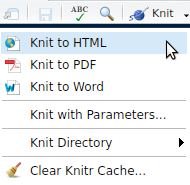
\includegraphics{images/knit.png}

\end{block}

\begin{block}{EXERCISE 4 \textbar{} Include another figure in your
report}

\begin{itemize}
\tightlist
\item
  If there's time\ldots{}
\item
  See \texttt{preliminary\_results\_summary.Rmd}
\end{itemize}

\end{block}

\begin{block}{EXERCISE 5 \textbar{} Create a new summary R Markdown
report}

Sometimes you may have to write multiple reports

\begin{itemize}
\tightlist
\item
  Name it something new and relevant
\item
  Save it in the same directory as helper.R
\item
  Delete everything after the first chunk.
\item
  Source to the same helper.R
\item
  Write some text and include a figure or table
\end{itemize}

\end{block}

\end{frame}

\begin{frame}{4. Writing a manuscript}
\protect\hypertarget{writing-a-manuscript}{}

\end{frame}

\begin{frame}

\begin{block}{Recap of recipe for a summary report:}

\begin{longtable}[]{@{}cc@{}}
\toprule
Ingredient & In this example\tabularnewline
\midrule
\endhead
data & starbucks\_drinkMenu\_expanded.csv\tabularnewline
helper script & helper.R\tabularnewline
R Markdown summary document &
preliminary\_results\_summary.Rmd\tabularnewline
\bottomrule
\end{longtable}

\end{block}

\end{frame}

\begin{frame}[fragile]

\begin{block}{Recipe for R Markdown .docx manuscript}

\begin{longtable}[]{@{}cc@{}}
\toprule
\begin{minipage}[b]{0.42\columnwidth}\centering
Ingredient\strut
\end{minipage} & \begin{minipage}[b]{0.52\columnwidth}\centering
In this example\strut
\end{minipage}\tabularnewline
\midrule
\endhead
\begin{minipage}[t]{0.42\columnwidth}\centering
\emph{data}\strut
\end{minipage} & \begin{minipage}[t]{0.52\columnwidth}\centering
\emph{starbucks\_drinkMenu\_expanded.csv}\strut
\end{minipage}\tabularnewline
\begin{minipage}[t]{0.42\columnwidth}\centering
\emph{helper script}\strut
\end{minipage} & \begin{minipage}[t]{0.52\columnwidth}\centering
\emph{helper.R}\strut
\end{minipage}\tabularnewline
\begin{minipage}[t]{0.42\columnwidth}\centering
R Markdown document(s)\strut
\end{minipage} & \begin{minipage}[t]{0.52\columnwidth}\centering
manuscript.Rmd, results.Rmd\strut
\end{minipage}\tabularnewline
\begin{minipage}[t]{0.42\columnwidth}\centering
\textbf{style reference .docx file} (specify styles in your Word
doc)\strut
\end{minipage} & \begin{minipage}[t]{0.52\columnwidth}\centering
custom\_reference.docx\strut
\end{minipage}\tabularnewline
\begin{minipage}[t]{0.42\columnwidth}\centering
\textbf{references in .bib format}\strut
\end{minipage} & \begin{minipage}[t]{0.52\columnwidth}\centering
starbucks\_refs.bib\strut
\end{minipage}\tabularnewline
\begin{minipage}[t]{0.42\columnwidth}\centering
\textbf{style bibliography (csl) file} (how your bibliography will be
formatted)\strut
\end{minipage} & \begin{minipage}[t]{0.52\columnwidth}\centering
apa.csl\strut
\end{minipage}\tabularnewline
\bottomrule
\end{longtable}

\end{block}

\begin{block}{Recipe for R Markdown manuscript: Caveat!}

\begin{itemize}
\tightlist
\item
  This is one (my) way of doing it
\item
  There are many other ways!
\item
  Many components are optional, for example:

  \begin{itemize}
  \tightlist
  \item
    style reference .docx file
  \item
    results.Rmd
  \end{itemize}
\item
  See resources at end of this presentation for inspiration!
\end{itemize}

\end{block}

\begin{block}{Recipe for R Markdown manuscript: Caveat!}

\begin{itemize}
\tightlist
\item
  While you \emph{can} be really specific in your formatting, we won't
  get into a \emph{ton} of detail here.
\item
  Since many journals often do a lot of the formatting from their end,
  what authors actually need to submit may be fairly bare-bones
  (sometimes)
\item
  If you're submitting a .docx file for publication, you can also make
  your final tweaks in the actual Word document itself, rather than in R
  Markdown

  \begin{itemize}
  \tightlist
  \item
    Save this until the end, because whatever you do in the Word
    document itself will be rewritten when you knit in R Markdown.
  \end{itemize}
\end{itemize}

\end{block}

\begin{block}{R Markdown document\emph{S} ?}

\textbf{manuscript.Rmd}

\begin{itemize}
\tightlist
\item
  The main text (intro, methods, discussion, references, etc\ldots{}
  Everything but results!)
\end{itemize}

\textbf{results.Rmd}

\begin{itemize}
\tightlist
\item
  Write your results in a separate .Rmd file, and knit it in as a
  \href{https://yihui.name/knitr/demo/child/}{child document}
\end{itemize}

\textbf{Benefits:}

\begin{itemize}
\tightlist
\item
  Cleaner!
\item
  Makes it easier to organize your writing
\end{itemize}

\end{block}

\begin{block}{manuscript.Rmd}

We will start with the main body file

\begin{itemize}
\tightlist
\item
  Open manuscript.Rmd
\item
  Knit it!
\item
  Examine it 🔍
\end{itemize}

\end{block}

\begin{block}{Manuscript: YAML}

We can make use of many more options!

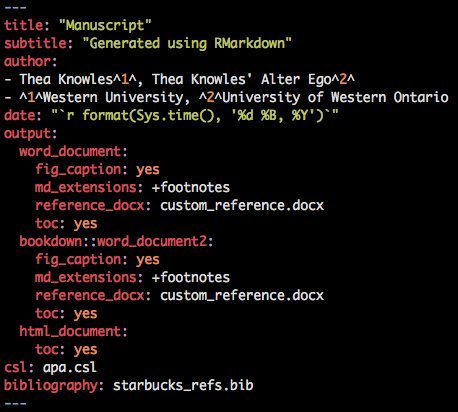
\includegraphics{images/manuscript_yaml.png}

\end{block}

\begin{block}{Manuscript: YAML}

Let's focus on the word\_document output for now

\begin{itemize}
\tightlist
\item
  See more options in
  \href{https://rmarkdown.rstudio.com/word_document_format.html}{RStudio's
  R Markdown overview}
\end{itemize}

\end{block}

\begin{block}{custom\_reference.docx}

\begin{itemize}
\tightlist
\item
  Allows you to set the styles for your .docx output in Microsoft Word
  directly
\item
  Contents of the .docx file are IGNORED
\item
  Styles and properties (margins, headers text, etc) are used in .Rmd's
  .docx output
\item
  For easiest use, include the custom\_reference.docx in the same
  directory as the rest of your RProject
\end{itemize}

\end{block}

\begin{block}{EXERCISE 6 \textbar{} Modify styles in
custom\_reference.docx}

\begin{itemize}
\tightlist
\item
  Make Header 1 size 16 font
\item
  Make Header 2 \emph{italicized}
\item
  Add page numbers
\item
  Knit manuscript.Rmd again and see what changed.
\end{itemize}

\end{block}

\begin{block}{Manuscript: YAML \textbar{} Markdown extensions}

\texttt{md\_extensions:\ +footnotes}

\begin{itemize}
\tightlist
\item
  See the \href{http://pandoc.org/MANUAL.html\#extensions}{Pandoc
  manual} to learn more.
\item
  So far: I've just use it for footnotes! 👣
\end{itemize}

\end{block}

\begin{block}{Bibliography info}

\end{block}

\begin{block}{Bibliography info: starbucks\_refs.bib}

References in BibLaTex (.bib) format: \texttt{starbucks\_refs.bib}

\begin{itemize}
\item
  Use .bib format

  \begin{itemize}
  \tightlist
  \item
    \href{http://www.bibtex.org/Using/}{About bibtex}
  \end{itemize}
\item
  Use another reference manager? No problem! Most can easily convert to
  .bib

  \begin{itemize}
  \tightlist
  \item
    \href{https://blog.mendeley.com/2012/03/24/how-to-series-generate-bibtex-files-for-your-collections-for-use-in-latex-part-3-of-12/}{Converting
    from Mendeley to .bib}
  \end{itemize}
\item
  Use \emph{keys} to cite a work in the markdown text, which will look
  like this in your markdown text:

  \begin{quote}
  \emph{``It is well known that some things are facts, and others are
  not {[}@knowles2018{]}.''}
  \end{quote}
\end{itemize}

\end{block}

\begin{block}{Bibliography info: starbucks\_refs.bib}

\begin{itemize}
\tightlist
\item
  A very useful RStudio Add-in that allows you to cite your sources from
  a drop-down menu: \href{https://github.com/crsh/citr}{citr}
\end{itemize}

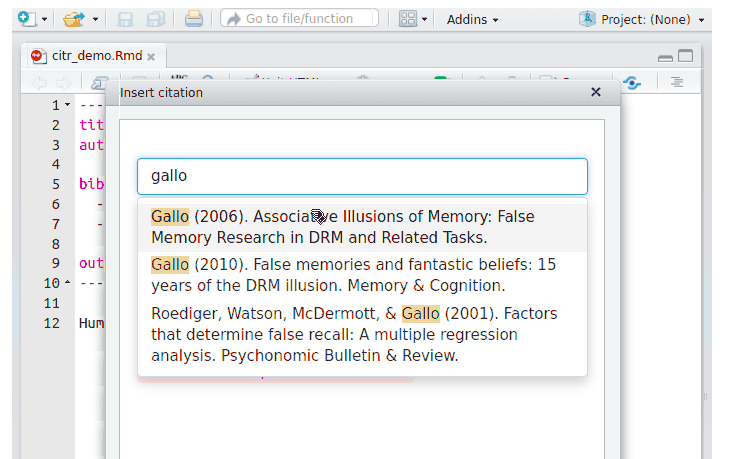
\includegraphics{images/citr.png}

\end{block}

\begin{block}{Bibliography info: Caveat!}

Thea's preferences here, full disclosure:

\begin{itemize}
\tightlist
\item
  I use one ``master'' references.bib file for all my projects
\item
  This file stays in one location, and I include the path to it in the
  YAML: \texttt{bibliography:\ /Users/thea/references.bib}
\item
  My ``keys'' all have the same format in order to make it easy to
  remember: firstauthorYEAR (knowles2018)

  \begin{itemize}
  \tightlist
  \item
    additional keyword if multiples (knowles2018dbs)
  \end{itemize}
\end{itemize}

\end{block}

\begin{block}{Bibliography info: Caveat!}

Thea's preferences here, full disclosure:

\begin{itemize}
\tightlist
\item
  When I come across a new paper, I immediately add its info to my .bib
  file
\item
  I get the bibtex info using Google Scholar's citation tools
  (specifically, the
  \href{https://chrome.google.com/webstore/detail/google-scholar-button/ldipcbpaocekfooobnbcddclnhejkcpn?hl=en}{GoogleScholar
  Chrome plugin})
\item
  I use \href{https://sourceforge.net/projects/jabref/}{JabRef} to
  manage my .bib file because I find it more user friendly, but you
  could also edit the .bib file in any text editor (just be cautious of
  formatting!)
\end{itemize}

\end{block}

\begin{block}{CSL file: apa.csl \textbar{} \textbf{CSL}: Citation Style
Language}

\begin{itemize}
\tightlist
\item
  Specifies how you want citations and bibliography formatted
\item
  Downloadable from many sources

  \begin{itemize}
  \tightlist
  \item
    \textbf{One good source}:
    \href{https://www.zotero.org/styles}{Zotero style repository}
  \end{itemize}
\item
  .csl files I use often:

  \begin{itemize}
  \tightlist
  \item
    \texttt{apa.csl}
  \item
    \texttt{biomed-central.csl}

    \begin{itemize}
    \tightlist
    \item
      when I need numeric in-text citations
    \end{itemize}
  \item
    \texttt{chicago-annotated-bibliography.csl}

    \begin{itemize}
    \tightlist
    \item
      when I'm writing annotated bibliographies
    \end{itemize}
  \end{itemize}
\end{itemize}

\end{block}

\end{frame}

\begin{frame}{Writing the manuscript body}
\protect\hypertarget{writing-the-manuscript-body}{}

\begin{block}{Writing the manuscript body}

\begin{itemize}
\tightlist
\item
  Write just as you did for the summary document:

  \begin{itemize}
  \tightlist
  \item
    Markdown-styled text, and R chunks sprinkled throughout!
  \end{itemize}
\item
  Separate writing tasks: ``story writing'' versus ``results reporting''
\end{itemize}

\end{block}

\end{frame}

\begin{frame}[fragile]{Inserting figures and tables \textbar{} Not
data-related!}
\protect\hypertarget{inserting-figures-and-tables-not-data-related}{}

\begin{block}{Inserting figures and tables}

\begin{itemize}
\tightlist
\item
  You can insert tables and figures in R chunks, as we did in the
  summary document
\item
  You can also insert them as non-R elements that wouldn't be accessible
  from the data

  \begin{itemize}
  \tightlist
  \item
    e.g., Participant demographics
  \end{itemize}
\end{itemize}

\end{block}

\begin{block}{Inserting tables in Markdown \textbar{} i.e., not R code}

\begin{itemize}
\tightlist
\item
  Markdown tables have a pretty straightforward syntax:
\end{itemize}

\begin{itemize}
\tightlist
\item
  Nevertheless, I often forget it. This site is handy:

  \begin{itemize}
  \tightlist
  \item
    \href{http://www.tablesgenerator.com/markdown_tables}{Table
    generator}
  \end{itemize}
\end{itemize}

\end{block}

\begin{block}{Inserting images in Markdown \textbar{} i.e., not R code}

Several ways to do this! Here are a few:

\begin{itemize}
\item
  Have a subdirectory called \texttt{images}; store your
  non-data-related images here
\item
  \texttt{!{[}Caption{]}(images/image1.png)} 
\end{itemize}

\end{block}

\begin{block}{Inserting tables in R chunks}

Just like how we did it in our summary report!

However: there are many more options within \texttt{kable()}

\begin{itemize}
\tightlist
\item
  See
  \href{https://cran.r-project.org/web/packages/kableExtra/vignettes/awesome_table_in_html.html}{kable
  documentation}
\end{itemize}

\end{block}

\end{frame}

\begin{frame}[fragile]{Writing the manuscript results \textbar{}
results.Rmd}
\protect\hypertarget{writing-the-manuscript-results-results.rmd}{}

\begin{block}{Writing the manuscript results \textbar{} results.Rmd}

\end{block}

\begin{block}{Including results as child file}

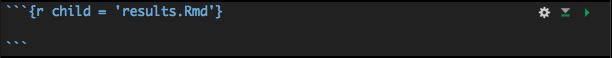
\includegraphics{images/child.png}

\begin{itemize}
\tightlist
\item
  YAML in the child document doesn't matter; it will inherit the YAML
  from the ``parent'' (main) .Rmd document

  \begin{itemize}
  \tightlist
  \item
    However, it may be helpful to include enough in the results.rmd YAML
    to be able to compile it on its own. That way, you can see what the
    results look like without having to knit the whole manuscript.
  \end{itemize}
\item
  Source your helper.R file
\end{itemize}

\end{block}

\begin{block}{Embedding figures}

\begin{itemize}
\tightlist
\item
  Just like in the summary document, but we can add more options to the
  chunk
\end{itemize}

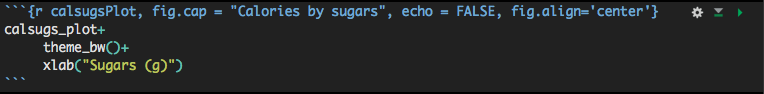
\includegraphics{images/fig_chunk.png}

\begin{itemize}
\tightlist
\item
  We will refer to the figure by its chunk label \texttt{calsugsPlot}
\item
  The caption will be specified by \texttt{fig.cap}
\item
  The figure number can be automatically added, but this requires an
  extra step for Word document outputs.
\end{itemize}

\end{block}

\begin{block}{Cross-referencing figures}

Unforunately, the standard word\_document output doesn't allow for us to
cross-reference Figures and Tables. You can still refer to Tables and
Figures in the text, but you have to do it manually (i.e., explicitly
type Figure 1, Table 2, etc.)

\emph{But\ldots{} there's good news}

\end{block}

\begin{block}{Cross-referencing figures \textbar{} Solution: Bookdown!}

\begin{itemize}
\tightlist
\item
  In the YAML, we can specify a new kind of output:
  \href{https://bookdown.org/yihui/bookdown/a-single-document.html}{\texttt{bookdown::word\_document2}}
\item
  This will allow us to automatically refer to Figures/Tables without
  having to explicitly refer to them by number

  \begin{itemize}
  \tightlist
  \item
    This is helpful if you wind up moving things around in your
    manuscript.
  \end{itemize}
\item
  You must be sure to Knit using word\_document2 output!
\end{itemize}

\end{block}

\begin{block}{Cross-referencing figures}

Syntax for cross-referencing with Bookdown::word\_document2 output:

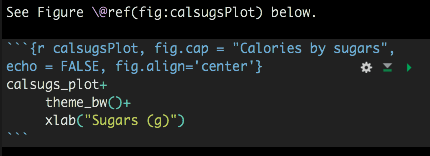
\includegraphics{images/fig_xref.png}

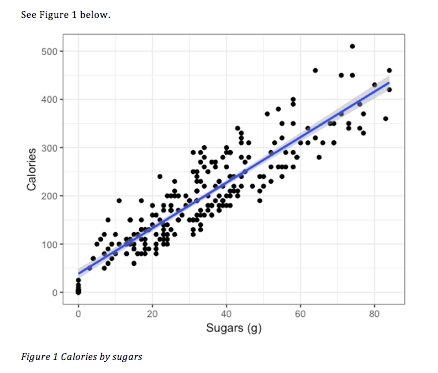
\includegraphics{images/fig_xref_output.png}

\end{block}

\begin{block}{EXERCISE 7 \textbar{} Uncomment the child input line and
knit the whole manuscript}

\end{block}

\begin{block}{MORE EXERCISES}

\begin{itemize}
\item
  Write a sentence in the results.Rmd that cites the article in the .bib
  file entitled ``Fat and sugar: an economic analysis''

  \begin{itemize}
  \tightlist
  \item
    Then knit the whole manuscript again
  \end{itemize}
\item
  Create a new figure with a label and a caption, then reference it in a
  new sentence.
\item
  Make a new manuscript from scratch and set up the Intro, Methods,
  Results, Discussion, and References.
\end{itemize}

\end{block}

\begin{block}{More to learn}

\begin{itemize}
\tightlist
\item
  Further customization of YAML

  \begin{itemize}
  \tightlist
  \item
    Author affiliations
  \item
    Abstract, keywords, etc
  \end{itemize}
\item
  Working with collaborators who don't use R Markdown

  \begin{itemize}
  \tightlist
  \item
    incorporating tracked changes?
  \item
    \href{https://stackoverflow.com/questions/35945728/ms-word-track-changes-and-rmarkdown}{This
    doesn't seem to have an answer yet}
  \end{itemize}
\item
  Incorporating
  \href{https://rmarkdown.rstudio.com/html_document_format.html\#custom_css}{css
  styles}
\item
  Fig/Table cross-referencing outside of results\ldots{} the answer's
  out there somewhere\ldots{}
\item
  \href{https://github.com/ropenscilabs/gramr}{Grammar check in R!}
\end{itemize}

\end{block}

\begin{block}{More to learn}

\begin{itemize}
\tightlist
\item
  It's okay to Google. Lots.
\item
  It's okay to be hacky at times to \emph{just do the thing}

  \begin{itemize}
  \tightlist
  \item
    Efficiency and elegance come with time

    \begin{itemize}
    \tightlist
    \item
      Well, sometimes the elegance lags behind
    \end{itemize}
  \end{itemize}
\end{itemize}

\end{block}

\begin{block}{Specific journal templates for R Markdown}

\url{https://github.com/rstudio/rticles}

\end{block}

\end{frame}

\begin{frame}{Awesome resources}
\protect\hypertarget{awesome-resources}{}

\begin{itemize}
\item
  \href{https://datascienceplus.com/r-for-publication-by-page-piccinini-lesson-1-r-basics/}{Page
  Piccinini's R for Publication Lessons}

  \begin{itemize}
  \tightlist
  \item
    Also contains GREAT explanations of regression analyses
  \end{itemize}
\item
  \href{https://rosannavanhespenresearch.wordpress.com/2016/02/03/writing-your-thesis-with-r-markdown-1-getting-started/}{Rosanna
  Van Hespen's guide to writing your thesis with R Markdown}
\item
  \href{https://www.one-tab.com/page/d00HO6mxTTuqo2o7aGCffQ}{A list of
  other very helpful resources}
\end{itemize}

\end{frame}

\end{document}
